The computational and communication costs incurred during training are integral to evaluating federated learning methods.
Personalized federated learning methods, in particular, often demand increased computation and memory resources.
In this context, we draw attention to the cost implications of various methods.
As depicted in Figure~\ref{fig: costs}, FedDecay exhibits comparable computational costs to other FL techniques.
The cost of learning rate scheduling is negligible per iteration, and the potential increase in communication rounds due to decaying updates does not meaningfully affect computation. 
In our experiments, FedDecay returns an identical cost to FedAvg for FEMNIST and SST2, which terminate in the same number of epochs.
FedDecay achieves similar or superior results without considerably higher communication and computation costs.
\begin{figure}[htbp]
    \centering
    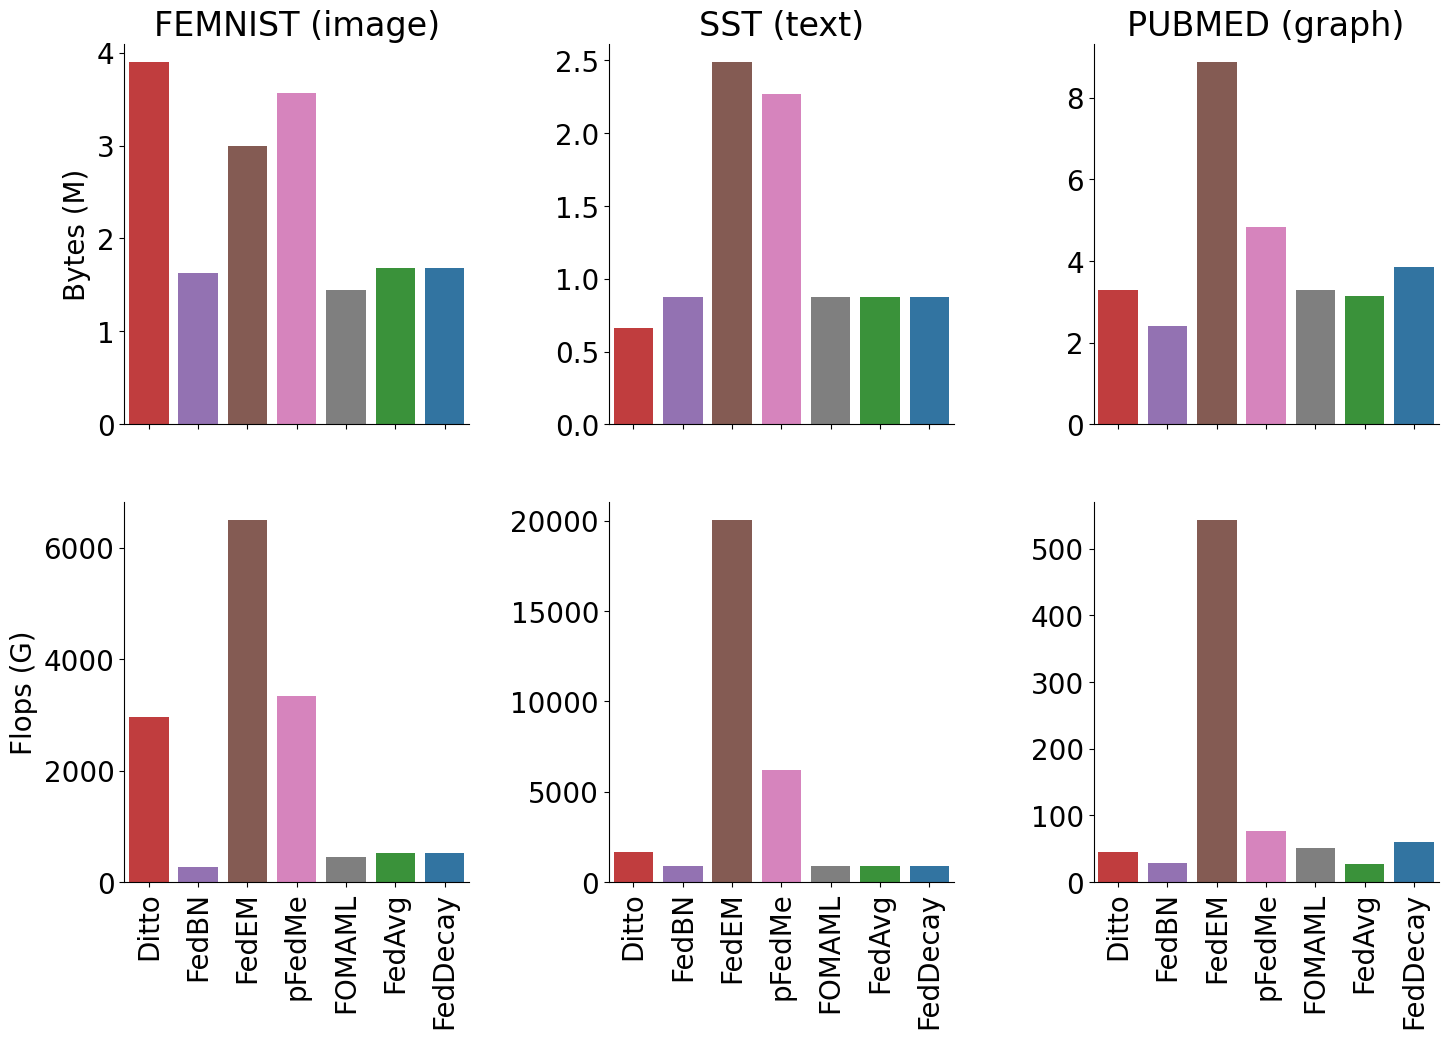
\includegraphics[width=.75\linewidth]{images/method-costs.png}
    \caption{
        Computational And Memory Costs.
        Total bytes communication (\textit{top}) and total floating point operations (\textit{bottom}) performed by the best-performing run of each method.
        FedDecay requires similar costs to other FL techniques, like FedAvg.
        Furthermore, FedDecay incurs considerably lower costs than personalized methods, especially FedEM and pFedMe.
    }
    \label{fig: costs}
\end{figure}

FedDecay requires substantially less memory and computation than FedEM and pFedMe, the two personalized methods that occasionally outperformed FedDecay in Section~\ref{sec: decay-exp-gen}.
Although FedDecay does not consistently outperform personalized federated learning methods, it is much more computationally efficient. 
It often dramatically closes the gap between other FL methods and personalized federated learning solutions.
This realization emphasizes FedDecay's efficiency in striking a favorable balance between performance and resource utilization, making it an attractive solution for practical federated learning scenarios.